
\chapter{Intuitions sur les espaces de fonctions}

Ce cours se veut volontairement informel sur nombre de points mathématiques. Il passe sous silence de nombreuses hypothèses et ne formalise pas les espaces de fonctions \footnote{\url{https://fr.wikipedia.org/wiki/Espace_fonctionnel}} ni les distributions \footnote{\url{https://fr.wikipedia.org/wiki/Distribution_(mathématiques)}}, par exemple, alors qu'il les manipule. Quand on passe à la mise en oeuvre informatique (numérique et discrétisée) des concepts traités dans ce cours, beaucoup de ces difficultés ne se posent néanmoins plus.

\section{Composition-décomposition de vecteurs dans \texorpdfstring{$\RR^n$}{\pdfRR\superscriptn}}

\subsection{L'espace vectoriel \texorpdfstring{$\RR^n$}{\pdfRR\superscriptn}, décomposition dans la base canonique}

On a l'habitude de se représenter de façon géométrique des vecteurs dans $\RR^n$ et de les manipuler (par exemple, les ajouter). En particulier, considérant $\RR^n$ comme un espace vectoriel et disposant d'une base $(e_1,....,e_n)$ dans cet espace (la base canonique ou une autre), l'algèbre linéaire établit qu'on peut fabriquer n'importe quel vecteur $u$ de $\RR^n$ en construisant une combinaison linéaire des vecteurs de cette base (ici les $a_i$ sont des réels):
\begin{equation}
u=a_1.e_1+\dots+a_n.e_n
\label{eq:decomposition_lineaire}
\end{equation} 
Il est également établi que cette combinaison linéaire est unique, c.a.d. qu'étant donné un vecteur $u$ et une base $(e_1,....,e_n)$, il existe un et un seul ensemble de coefficients $(a_1,....,a_n)$ tel que $u=a_1.e_1+\dots+a_n.e_n$.

\subsection{Décomposition d'un vecteur dans une base quelconque}

\subsubsection{Par résolution d'un sytème linéaire}

Etant donné un vecteur $u$ dans $\RR^n$, on peut avoir besoin de récupérer les coefficients $a_i$ de la décomposition de $u$ dans une base donnée.
 S'il s'agit de la base canonique, ces coefficients sont simplement les composantes du vecteur. S'il s'agit d'une autre base, cela peut, par exemple, se faire en résolvant un système de $n$ équations à $n$ inconnues (qui sont les $a_i$).

Par exemple, soit le vecteur $u=(5,3)^T$. Il se décompose sur la base canonique comme  
\begin{equation}
\begin{pmatrix} 5 \\ 3 \end{pmatrix} = 5  \begin{pmatrix} 1 \\ 0 \end{pmatrix} + 3  \begin{pmatrix} 0 \\ 1 \end{pmatrix}
\end{equation}
On peut identifier $a_1=5$ et $a_2=3$ immédiatement.

Si on souhaite décomposer $u$ sur une autre base, par exemple la base formée par les vecteurs $e_1=(1,1)^T$ et $e_2=(-1,1)^T$, pour identifier $a_1$ et $a_2$, il faut résoudre
\begin{equation}
\begin{pmatrix} 5 \\ 3 \end{pmatrix}  = a_1  \begin{pmatrix} 1 \\ 1 \end{pmatrix} + a_2  \begin{pmatrix} -1 \\ 1 \end{pmatrix}
\end{equation}
En écrivant cette équation comme 2 équations à 2 inconnues, on trouve rapidement $a_1=4$ et $a_2=-1$.

\subsubsection{Par projections orthogonales}

Regardons maintenant comment on peut obtenir les coefficients de la décomposition d'un vecteur $u$ sur une base de $\RR^n$, en utilisant des projections orthogonales. 

$\RR^n$ est un espace vectoriel, ce qui permet de faire des combinaisons linéaires de vecteurs, comme ci-dessus. Pour faire des projections orthogonales, il faut enrichir notre espace vectoriel avec un opérateur: le \textbf{produit scalaire}. Dans $\RR^n$, notons $\langle u , v \rangle$ le produit scalaire entre deux vecteurs $u=(u_1,\dots,u_n)$ et $v=(v_1,\dots,v_n)$. La définition simple du produit scalaire dans $\RR^n$ est : 
\begin{equation}
\langle u , v \rangle = \sum_{i=1}^n u_i.v_i
\end{equation}
La \textbf{norme euclidienne} $\|u\|$ d'un vecteur $u=(u_1,\dots,u_n)$ de $\RR^n$, qui décrit intuitivement sa longueur indépendamment de son orientation, est définie à partir du produit scalaire $\langle u, u \rangle$ comme 
\begin{equation}
\|u\|= \sqrt{\langle u, u \rangle}=\sqrt{\sum_i u_i^2}
\end{equation}

Le produit scalaire entre deux vecteurs $u$ et $v$ de $\RR^n$, tels qu'il y a un angle $\theta$ entre $u$ et $v$, peut se calculer comme:
\begin{equation}
\langle u, v \rangle=\|u\|.\|v\|cos(\theta)
\end{equation}
Autrement dit, l'\textbf{angle}, du moins ce que peut en déterminer son cosinus, est calculable comme le produit scalaire normalisé par la longueur des vecteurs impliqués dans ce produit scalaire :
\begin{equation}
cos(\theta) = \frac{\langle u, v \rangle}{\|u\|.\|v\|}
\end{equation}

Le produit scalaire permet aussi d'introduire la notion de \textbf{projection orthogonale} d'un vecteur de $\RR^n$ sur un autre. De façon générale, la projection orthogonale d'un vecteur $u$ sur un vecteur $v$ consiste à décomposer $u$ comme la somme d'un vecteur $u$ colinéaire à $v$, noté $u_{\| v}$ (dite "projection orthogonale de $u$ sur $v$") et une partie orthogonale à $v$, notée $u_{\perp v}$. Cette décomposition est unique (on n'en fait pas la démonstration ici).

%La projection d'un vecteur $u$ quelconque sur un vecteur $e_1$ de la base permet de récupérer directement le coefficient $a_1$ associé. 

Appliquons la projection orthogonale au cas où on projete $u$ sur chacun des vecteurs $e_i$ de la base, tour à tour. Prenons ci-dessous le cas de la projection sur $e_1$, le premier vecteur de la base. On s'intéresse à la décomposition de $u$ comme la somme d'un vecteur colinéaire à $e_1$ (dit "projection orthogonale de $u$ sur $e_1$"), noté $u_{\| e_1}$ et d'un vecteur orthogonal à $e_1$, notée $u_{\perp e_1}$.

\begin{equation}
u = \underbrace{\quad u_{\| e_1} \quad}_{\text{projection orthogonale de $u$ sur $e_1$}} + \underbrace{\quad u_{\perp e_1}}_{\text{composante orthogonale à $e_1$ }} \quad
\end{equation}

\begin{center} 
\begin{tikzpicture} [scale=3, axis/.style={->,blue,thick}, vector/.style={-stealth,red,very thick}, 
vector guide/.style={->,dashed,red,thick}]

%standard tikz coordinate definition using x, y, z coords


%tikz-3dplot coordinate definition using x, y, z coords

\pgfmathsetmacro{\ax}{0.8}
\pgfmathsetmacro{\ay}{0.8}
\pgfmathsetmacro{\az}{0.8}

\coordinate (O) at (0,0,0);
\coordinate (P) at (1,0,0);
\coordinate (Q) at (3,1,0);
\coordinate (M) at (3,0,0);
\coordinate (N) at (3,0.74*\ay,0.5*\az);

\draw[axis]   (O) -- (P) node[anchor=north east]{$e_1$};
\draw[vector] (O) -- (Q) node[anchor=south]{$u$}; ; 
\draw[vector guide] (M) -- (Q) node[anchor=north west]{$u_{\perp e_1}$};
%\draw[vector guide]  (P) -- (M);
\draw[vector guide]         (O) -- (M) node[anchor= north east]{$u_{\|e_1}$};

\end{tikzpicture}
\end{center} 

Dans le triangle rectangle, on a :

\begin{equation}
\langle u , e_1 \rangle   = \|u\|.\|e_1\|cos(\widehat{u,e_1})  =  \|u_{\|e_1}\|.\|e_1\| = \langle u_{\|e_1},e_1 \rangle
\end{equation}


Cela nous permet de caractériser la longueur du vecteur $u_{\|e_1}$ : 

\begin{equation}
\|u_{\|e_1}\|  = \frac{\langle u , e_1 \rangle}{\|e_1\|}
\end{equation}

Par ailleurs, comme $u$ et $e_1$ sont colinéaires, on a 
\begin{equation}
u_{\|e_1} = \|u_{\|e_1}\| . \frac{e_1}{\|e_1\|}
\end{equation}

Si bien qu'en conclusion, on peut exprimer $u_{\|e_1}$ en fonction de $e_1$ et identifier le coefficient $a_1$.
\begin{equation}
u_{\|e_1} = \frac{\langle u , e_1 \rangle}{\|e_1\|^2} \quad e_1
\end{equation}

Si les $e_i$ sont orthogonaux deux à deux, c.a.d. qu'on a une \textbf{base orthogonale}, alors on a plus généralement :
\begin{equation}
u = \frac{\langle u , e_1 \rangle}{\|e_1\|^2} \quad e_1 +\dots + \frac{\langle u , e_n \rangle}{\|e_n\|^2} \quad e_n 
\end{equation}
qui est une nouvelle manière d'écrire l'équation (\ref{eq:decomposition_lineaire}) qui donne un moyen de calcul direct des coefficients $a_i$ de la décomposition, grâce au produit scalaire.

Appliquons cela à l'exemple vu plus haut $u=(5,3)^T$ à décomposer sur la base $e_1=(1,1)^T$ et $e_2=(-1,1)^T$ , et on retrouve bien les résultats qu'on avait obtenus par résolution du système linéaire :
\begin{equation*}
a_1=\frac{\langle u , e_1 \rangle}{\|e_1\|^2} = \frac{\langle\begin{pmatrix} 5 \\ 3 \end{pmatrix},\begin{pmatrix} 1 \\ 1 \end{pmatrix}\rangle}{\sqrt{1^2+1^2}^2}=4 \quad \text{et} \quad a_2=\frac{\langle u , e_2 \rangle}{\|e_2\|^2} = \frac{\langle\begin{pmatrix} 5 \\ 3 \end{pmatrix},\begin{pmatrix} -1 \\ 1 \end{pmatrix}\rangle}{\sqrt{(-1)^2+1^2}^2}=-1 
\end{equation*}

Si, de plus, on considère le cas particulier où $\|e_i\|=1$ pour tout $i \in \{1,...,n\}$ (c.a.d. la base est \textbf{orthonormée} en plus d'être orthogonale), alors c'est encore plus simple :
\begin{equation}
u = \langle u , e_1 \rangle ~e_1 +\dots + \langle u , e_n \rangle ~e_n 
\end{equation}

\section{Mêmes notions, mais sur des fonctions}

La raison de tous les rappels ci-dessus est que l'analyse de Fourier travaille sur des concepts analogues, sinon que les éléments de l'espace sont des fonctions au lieu d'être des vecteurs de $\RR^n$. Par exemple, la figure ~\ref{fonctions_orthogonales} illustre comment la combinaison linéaire de quelques fonctions élémentaires (ici trinométriques) permettrait de générer des fonctions très diverses.

%\tdplotsetmaincoords{60}{120} 

\begin{figure}[H]
\begin{center}
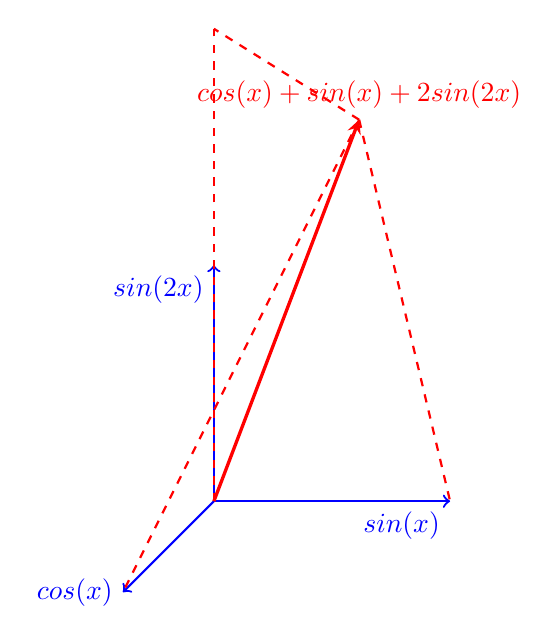
\begin{tikzpicture} [scale=3, axis/.style={->,blue,thick}, vector/.style={-stealth,red,very thick}, 
vector guide/.style={dashed,red,thick}]

%standard tikz coordinate definition using x, y, z coords
\coordinate (O) at (0,0,0);

%tikz-3dplot coordinate definition using x, y, z coords

\pgfmathsetmacro{\ax}{0.8}
\pgfmathsetmacro{\ay}{0.8}
\pgfmathsetmacro{\az}{0.8}

\coordinate (P) at (\ax,\ay,\az);

%draw axes
\draw[axis] (0,0,0) -- (1,0,0) node[anchor=north east]{$sin(x)$};
\draw[axis] (0,0,0) -- (0,1,0) node[anchor=north east]{$sin(2x)$};
\draw[axis] (0,0,0) -- (0,0,1) node[anchor=east]{$cos(x)$};

%draw a vector from O to P
\draw[vector] (0,0,0) -- (1,2,1) node[anchor=south]{$cos(x)+sin(x)+2sin(2x)$}; ; 

%draw guide lines to components
%\draw[vector guide]         (O) -- (\ax,\ay,0);
%\draw[vector guide] (\ax,\ay,0) -- (P);
%\draw[vector guide]         (P) -- (0,0,\az);
\draw[vector guide] (1,2,1) -- (0,0,1);
\draw[vector guide] (1,2,1) -- (1,0,0);
\draw[vector guide] (1,2,1) -- (0,2,0);
\draw[vector guide] (0,0,0) -- (0,2,0);
%\node[tdplot_main_coords,anchor=east]
%at (\ax,0,0){(\ax, 0, 0)};
%\node[tdplot_main_coords,anchor=west]
%at (0,\ay,0){(0, \ay, 0)};
%\node[tdplot_main_coords,anchor=south]
%at (\ax,0:ay,\az){(0, 0, \az)};
\end{tikzpicture}
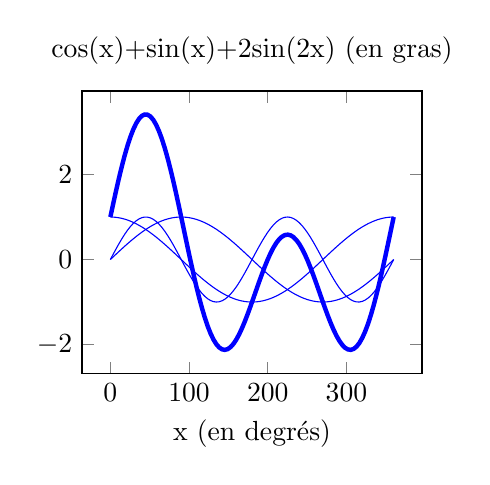
\begin{tikzpicture}
\begin{axis}[scale=0.63,xlabel={x (en degrés)},title={cos(x)+sin(x)+2sin(2x) (en gras) }]
 \addplot[domain=0:360, samples= 100, blue,  ultra thick]{cos(x)+sin(x)+2*sin(2*x)};
 \addplot[domain=0:360, samples= 100, blue]{cos(x)};
 \addplot[domain=0:360, samples= 100, blue]{sin(x)};
 \addplot[domain=0:360, samples= 100, blue]{sin(2*x)};
\end{axis}
\end{tikzpicture}
\end{center}
\caption{Représentation intuitive d'un espace de fonctions. Par exemple, la famille $(cos(x),sin(x),sin(2x))$ permet de générer une infinité de fonction par combinaison linéaire $a_1.cos(x)+a_2.sin(x)+a_3.sin(2x)$ où les $a_i \in \RR$. Par exemple, l'illustration correspond au cas (arbitraire) $a_1=1,a_2=1,a_3=2$.} Les courbes en trait fin sont cos(x), sin(x) et sin(2x).
\label{fonctions_orthogonales}
\end{figure}

Il reste utile de garder à l'esprit les interprétations géométriques qu'on a pour les vecteurs. On précise maintenant des adaptations des définitions et interprétations dans le cas des fonctions :

\subsection{Produit scalaire entre fonctions}
\label{sec:prodscal}

Soit l'espace $E$ sur $\RR$ des fonctions continues sur
$[a,b]$ vers $\RR$. Définissons un\footnote{``un'' et non ``le'' car
on pourrait en définir d'autres, mais celui-ci est de loin le plus usuel.} produit scalaire entre deux fonctions $f$ et $g$ de cet espace :
\begin{eqnarray}
E \times E & \rightarrow & \RR \nonumber \\
\langle f, g \rangle & \mapsto & \int_a^b f(x)\; g(x)\; dx
\end{eqnarray}

Le premier point à remarquer est que cette définition est semblable à cette qu'on a pour un produit scalaire usuel entre vecteurs : on fait la somme des produits sur les composantes du vecteurs - à ceci près que pour les fonctions cette somme est définie sur un espace continu  $[a,b]$ plutôt qu'un ensemble discret de composantes.

L'\textbf{orthogonalité} entre $f$ et $g$ correspond, comme dans $\RR^n$,
au cas où le produit scalaire s'annule :
\begin{equation}
\int_a^b f(x)g(x)=0
\end{equation}


La figure~\ref{premier_exemple} illustre trois exemples simples avec des fonctions orthogonales $f$ et $g$ définies sur $[-3,3]$. Sur ces exemples, les fonctions sont constantes par morceaux pour la commodité du calcul mental, mais de façon générale elles n'ont pas besoin d'être constantes par morceaux.

\begin{figure}
\begin{center}
\begin{tikzpicture}[background rectangle/.style={fill=olive!5}, show background rectangle]
\begin{groupplot}[group style={group size=1 by 3, horizontal sep=2cm, vertical sep=2cm}, xmax=3,ymin=-2,ymax=2,scale=0.6,axis lines=center,xtick distance=1]
\nextgroupplot[title={\textbf{$f(x)$}}]
  \addplot[domain=-3:0, blue, ultra thick] (x,1);
  \addplot[domain=0:3, blue,  ultra thick] (x,0);
\nextgroupplot[title={\textbf{$g(x)$}}]
  \addplot[domain=-3:0, blue, ultra thick] (x,0);
  \addplot[domain=0:3, blue,  ultra thick] (x,1);
\nextgroupplot[title={\textbf{$f(x)g(x)$}}]
  \addplot[domain=-3:0, blue, ultra thick] (x,0);
  \addplot[domain=0:3, blue,  ultra thick] (x,0);
\end{groupplot}
\end{tikzpicture}
\hfill 
\begin{tikzpicture}[background rectangle/.style={fill=olive!5}, show background rectangle]
\begin{groupplot}[group style={group size=1 by 3, horizontal sep=2cm, vertical sep=2cm}, xmax=3,ymin=-2,ymax=2,scale=0.6,axis lines=center,xtick distance=1]
\nextgroupplot[title={\textbf{$f(x)$}}]
  \addplot[domain=-3:0, blue, ultra thick] (x,1);
  \addplot[domain=0:3, blue,  ultra thick] (x,1);
\nextgroupplot[title={\textbf{$g(x)$}}]
  \addplot[domain=-3:0, blue, ultra thick] (x,-1);
  \addplot[domain=0:3, blue,  ultra thick] (x,1);
\nextgroupplot[title={\textbf{$f(x)g(x)$}}]
  \addplot[domain=-3:0, blue, ultra thick] (x,-1);
  \addplot[domain=0:3, blue, ultra thick] (x,1);
\end{groupplot}
\end{tikzpicture}
\hfill 
\begin{tikzpicture}[background rectangle/.style={fill=olive!5}, show background rectangle]
\begin{groupplot}[group style={group size=1 by 3, horizontal sep=2cm, vertical sep=2cm
}, xmax=3,ymin=-2,ymax=2,scale=0.6,axis lines=center,xtick distance=1]
\nextgroupplot[title={\textbf{$f(x)$}}]
  \addplot[domain=-3:0, blue, ultra thick] (x,1);
  \addplot[domain=0:3, blue,  ultra thick] (x,-1);
\nextgroupplot[title={\textbf{$g(x)$}}]
  \addplot[domain=-3:-1.5, blue,  ultra thick] (x,1);
  \addplot[domain=-1.5:0, blue, ultra thick] (x,-1);
  \addplot[domain=0:3, blue,  ultra thick] (x,1);
\nextgroupplot[title={\textbf{$f(x)g(x)$}}]
  \addplot[domain=-3:-1.5, blue, ultra thick] (x,1);
  \addplot[domain=-1.5:0, blue, ultra thick] (x,-1);
  \addplot[domain=0:3, blue, ultra thick] (x,-1);
\end{groupplot}
\end{tikzpicture}
\end{center}
\caption{Les trois colonnes correspondent à trois exemples. Dans les deux premiers cas, l'intégrale entre -3 et 3 du produit des fonctions est nulle, donc les fonctions sont orthogonales. Dans le troisième cas, le produit scalaire vaut -3.}
\label{premier_exemple}
\end{figure}

La définition plus générale du produit scalaire, qui englobe les cas particuliers des vecteurs dans $\RR^n$ et des fonctions, et qu'on pourrait appliquer à encore d'autres types d'objets mathématiques (matrices, ...) est qu'un produit scalaire doit vérifier les propriétés suivantes :

\begin{enumerate}
\item il s'agit d'une \emph{forme linéaire}, i.e. une application
  linéaire dont l'image $\in \RR$ (qui est le corps sur lequel est
  construit l'espace vectoriel dont proviennent $f$ et $g$),
\item cette forme est \emph{bilinéaire} et \emph{symétrique}
  (bilinéaire : linéaire vis-à-vis de $f$ et de $g$),
\item on dit que le produit scalaire est \emph{défini positif},
  c'est-à-dire :
\begin{enumerate}
\item $\forall f \in E, \langle f, f \rangle=\int_a^bf(x)^2 dx~\geq 0 $ 
\item $\langle f, f \rangle=\int_a^bf(x)^2 dx=0 \Longleftrightarrow f=0$
\end{enumerate}
\end{enumerate}
``Produit scalaire'' est donc une expression raccourcie de ``forme
bilinéaire symétrique définie positive''. 

La figure~\ref{exemples_produitscalaire} montre d'autres exemples.

\begin{figure}
\begin{center}
\begin{tikzpicture}[background rectangle/.style={fill=olive!5}, show background rectangle]
\begin{groupplot}[group style={group size=1 by 3},scale=0.55,domain=0:360, axis lines=center]
\nextgroupplot[title={\textbf{$f(x)=sin(x)$}}]
  \addplot[blue, ultra thick] {sin(x)};
\nextgroupplot[title={$g(x)=sin(x)$}]
  \addplot[blue, ultra thick] {sin(x)};
\nextgroupplot[title=$f(x).g(x)$]
  \addplot[cyan,fill,opacity=0.2,ultra thick] {sin(x)*sin(x)};
\end{groupplot}

\node[align=center,font=\bfseries, yshift=2em] (title) 
    at (current bounding box.north)
    {Exemple 1};

\end{tikzpicture}
\begin{tikzpicture}[background rectangle/.style={fill=olive!5}, show background rectangle]
\begin{groupplot}[group style={group size=1 by 3,horizontal sep=2cm, vertical sep=2cm}, scale=0.5,domain=0:360, axis lines=center]
\nextgroupplot[title={$f(x)=sin(x)$}]
  \addplot[blue, ultra thick] {sin(x)};
\nextgroupplot[title={$g(x)=cos(x)$}]
  \addplot[blue, ultra thick] {cos(x)};
\nextgroupplot[title=$f(x).g(x)$]
  \addplot[cyan,fill,opacity=0.13,ultra thick] {sin(x)*cos(x)};
\end{groupplot}
\node[align=center,font=\bfseries, yshift=2em] (title) 
    at (current bounding box.north)
    {Exemple 2};
\end{tikzpicture}
\begin{tikzpicture}[background rectangle/.style={fill=olive!5}, show background rectangle]
\begin{groupplot}[group style={group size=1 by 3,horizontal sep=2cm, vertical sep=2cm}, scale=0.5,domain=0:360, axis lines=center]
\nextgroupplot[title={$f(x)=sin(x)$}]
  \addplot[blue, ultra thick] {sin(x)};
\nextgroupplot[title={$g(x)=sin(2x)$}]
  \addplot[blue, ultra thick] {sin(2*x)};
\nextgroupplot[title=$f(x).g(x)$]
  \addplot[fill=cyan,opacity=0.13,text opacity=1] {sin(x)*sin(2*x)};
\end{groupplot}
\node[align=center,font=\bfseries, yshift=2em] (title) 
    at (current bounding box.north)
    {Exemple 3};
\end{tikzpicture}
\end{center}
\caption{La figure montre trois exemples (les trois colonnes) de produits scalaires entre fonctions. Les abscisses sont en degrés. Le résultat du produit scalaire est l'aire de la zone hachurée dans la 3eme rangée. Attention, ces aires sont à considérer avec leurs signes positif/négatif, c.a.d. que dans l'exemple 1 l'aire totale est positive tandis que dans les exemples 2 et 3 l'aire totale est nulle. Le premier cas est à rapprocher du calcul de la norme d'une fonction (qui elle-même ressemble au calcul de la norme d'un vecteur), tandis que les exemples 2 et 3 illustrent des cas d'orthogonalité, exemples les plus simples qu'on verra généralisables aux fonctions de base des séries de Fourier.}
\label{exemples_produitscalaire}
\end{figure}

\begin{figure}
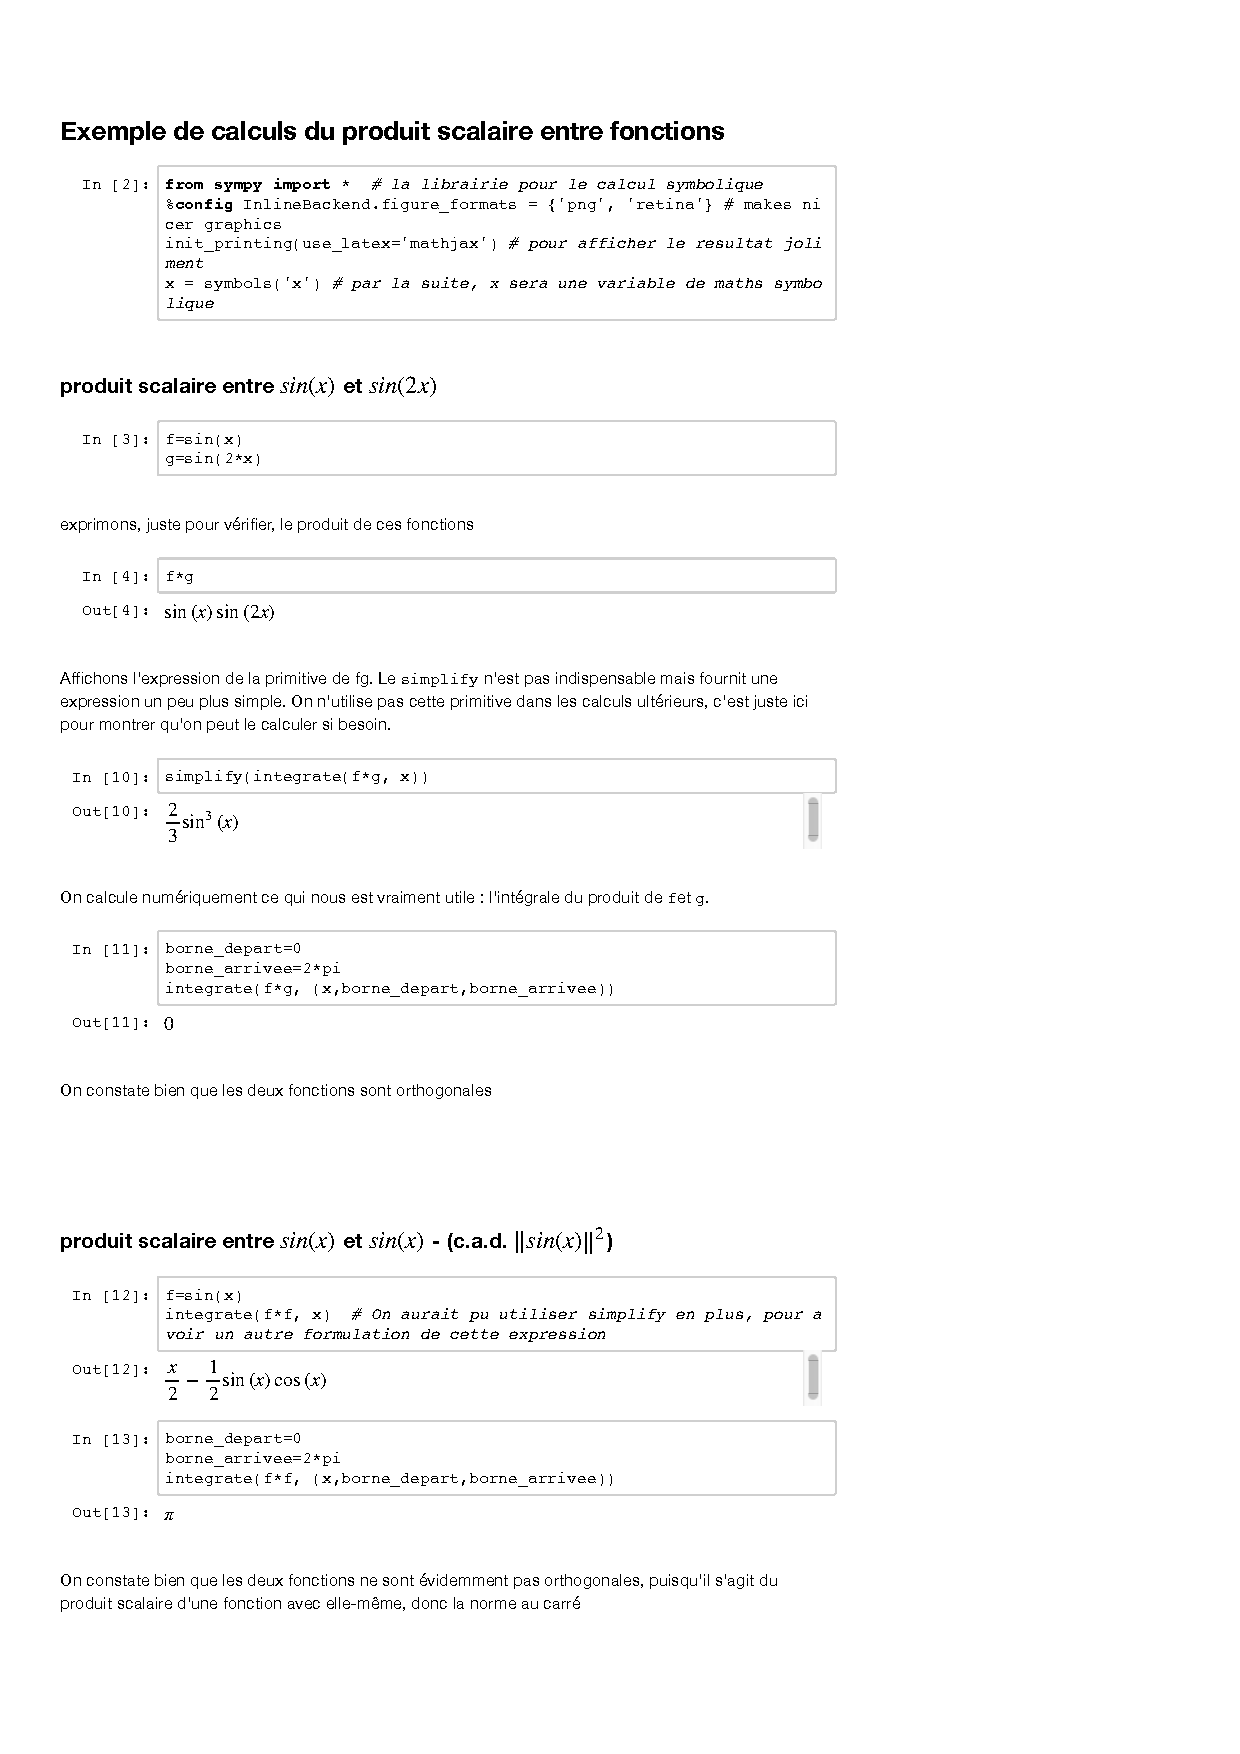
\includegraphics[scale=0.7]{fourier-notebook-polytech.pdf}
\caption{Exemple de calcul symbolique en python pour le calcul d'un produit scalaire entre fonctions.}
\end{figure}

\subsection{Norme d'une fonction}


De façon analogue aux vecteurs, on peut définir la norme (dite \emph{euclidienne}) d'une fonction $f$:
\begin{equation}
\|f\|= \sqrt{\langle f, f \rangle}=\sqrt{\int_a^b f(t)^2dt}
\end{equation} 

\subsection{Angle entre fonctions}


Une définition analogue aux vecteurs peut être construite pour l'angle entre deux fonctions $f$ et $g$:

\begin{equation}
cos(\theta) = \frac{\langle f, g \rangle}{\|f\|.\|g\|}
\end{equation}

%Soient trois vecteurs $v$, $u_1$ et $u_2$ dans $\RR^n$. On s'intéresse à la décomposition suivante :
%
%\begin{equation}
%v = \underbrace{\quad v_{\| u} \quad}_{\text{projection orthogonale de $u_1$ sur $v$}} + \underbrace{\quad v_{\perp u}}_{\text{composante orthogonale à $u$ }} \quad
%\end{equation}
%
%
%
%\begin{center} 
%\begin{tikzpicture} [scale=5, tdplot_main_coords, axis/.style={->,blue,thick}, 
%vector/.style={-stealth,red,very thick}, 
%vector guide/.style={dashed,red,thick}]
%
%%standard tikz coordinate definition using x, y, z coords
%\coordinate (O) at (0,0,0);
%
%%tikz-3dplot coordinate definition using x, y, z coords
%
%\pgfmathsetmacro{\ax}{0.8}
%\pgfmathsetmacro{\ay}{0.8}
%\pgfmathsetmacro{\az}{0.8}
%
%\coordinate (P) at (0.8*\ax,1*\ay,2*\az);
%
%%draw axes
%\draw[axis] (0,0,0) -- (1,0,0) node[anchor=north east]{$u_1$};
%\draw[axis] (0,0,0) -- (0,1,0) node[anchor=north west]{$u_2$};
%%\draw[axis] (0,0,0) -- (0,0,1.5) node[anchor=east]{};
%
%%draw a vector from O to P
%\draw[vector] (O) -- (P) node[anchor=south]{$v$}; ; 
%
%%draw guide lines to components
%
%\coordinate (M) at (0,0.74*\ay,0);
%\coordinate (N) at (0,0.74*\ay,0.5*\az);
%\coordinate (Q) at (0.5*\ax,0,0);
%\coordinate (R) at (0.5*\ax,0.74*\ay,0);
%\coordinate (S) at (0.0*\ax,0.0*\ay,0.9*\az);
%
%\draw[vector guide]         (N) -- (N) node[anchor=north west]{$v_{\perp u_2}$};
%
%\draw[vector guide]         (P) -- (M);
%\draw[axis]         (O) -- (M) node[anchor=north east]{$v_{\|u_2}$};
%\draw[axis]         (O) -- (Q) node[anchor=west]{$v_{\|u_1}$};
%\draw[axis]         (O) -- (R) node[anchor=north east]{$v_{\|u_1}+v_{\|u_2}$};
%\draw[vector guide]         (P) -- (Q); 
%\draw[vector guide]         (S) -- (S) node[anchor=south]{$v_{\perp u_1}$};
%\draw[vector guide]         (P) -- (R) node[anchor=north east]{$v_{\perp u_{1,2}}$};
%
%\end{tikzpicture}
%\end{center} 
%Caractérisons la longueur du vecteur $v_{\|u}$ : 
%
%\begin{equation}
%\langle u , v \rangle   = \langle u , v_{\|u} \rangle
%\end{equation}
%
%\begin{equation}
%\|u\|.\|v\|cos(\widehat{u,v})  =  \|u\|.\|v_{\|u}\|
%\end{equation}
%
%\begin{equation}
%\|v_{\|u}\|  = \frac{\langle u , v \rangle}{\|u\|}
%\end{equation}
%
%Le cas d'utilisation qui nous intéresse principalement ici est celui où $v$ est un vecteur quelconque et $u$ un vecteur de base (généralement parmi d'autres vecteurs de base), dont nous souhaitons déterminer la contribution à $v$ (par combinaison linéaire avec les autres vecteurs de base).
%
%Si $\|u\|=1$ (ce qui est le cas si $u$ est un des vecteurs d'une base orthonormée), alors $\|v_{\|u}\|  = \langle u , v \rangle$. Dans ce cas, la décomposition initiale peut s'écrire comme suit, où on voit que le produit scalaire fournit directement le coefficient associé à $u$ dans la combinaison linéaire.
%\begin{equation}
%v = \underbrace{\quad \langle u , v \rangle. u \quad}_{\text{projection orthogonale de $u$ sur $v$}} + \underbrace{\quad v_{\perp u}}_{\text{composante orthogonale à $u$ }} \quad
%\end{equation}
